\AtBeginSection[]{
	\begin{frame}
		\vfill
		\centering
		\begin{beamercolorbox}[sep=8pt,center,shadow=false,rounded=true]{title}
			\usebeamerfont{title}\insertsectionhead\par% 
		\end{beamercolorbox}
		    \tableofcontents[currentsubsection] 
		\vfill
	\end{frame}
}

\section{Simulation noVAPOR}

\begin{frame}{Simulation noVAPOR}
	
\begin{itemize}
	\item No vapor is written, bc no condensation and dry atmosphere we also don't want to take into effect the light air particles that are humid. 
	\item Strong inversion 
	\item open boundaries to have constant wind and test if rolls stay
	\item Big domain to have formation of rolls but costly
\end{itemize}

\begin{figure}
	
\includegraphics[width=0.4\textheight]{FIGURES/noVAPOR/inputs.png}
\end{figure}

\end{frame}

\subsection{Profiles vitesses}
\begin{frame}{Profiles}
Tjs pb des vents verticaux en altitude + CL se stabilise (peut etre du a temperétaure au sol plus faible que profil de temp dans mNH)
	\begin{figure}[t]
		\centering
		
\includegraphics[width=0.8\textwidth]{FIGURES/noVAPOR/wind_profiles.png}
	\end{figure}
\end{frame}

\subsection{Flux}
\begin{frame}{Flux}
Flux sensible cohérent avec papier de Wahiba ; un peu trop forts ($\approx 100W.m^{-2}$)
	\begin{figure}[t]
		\centering
		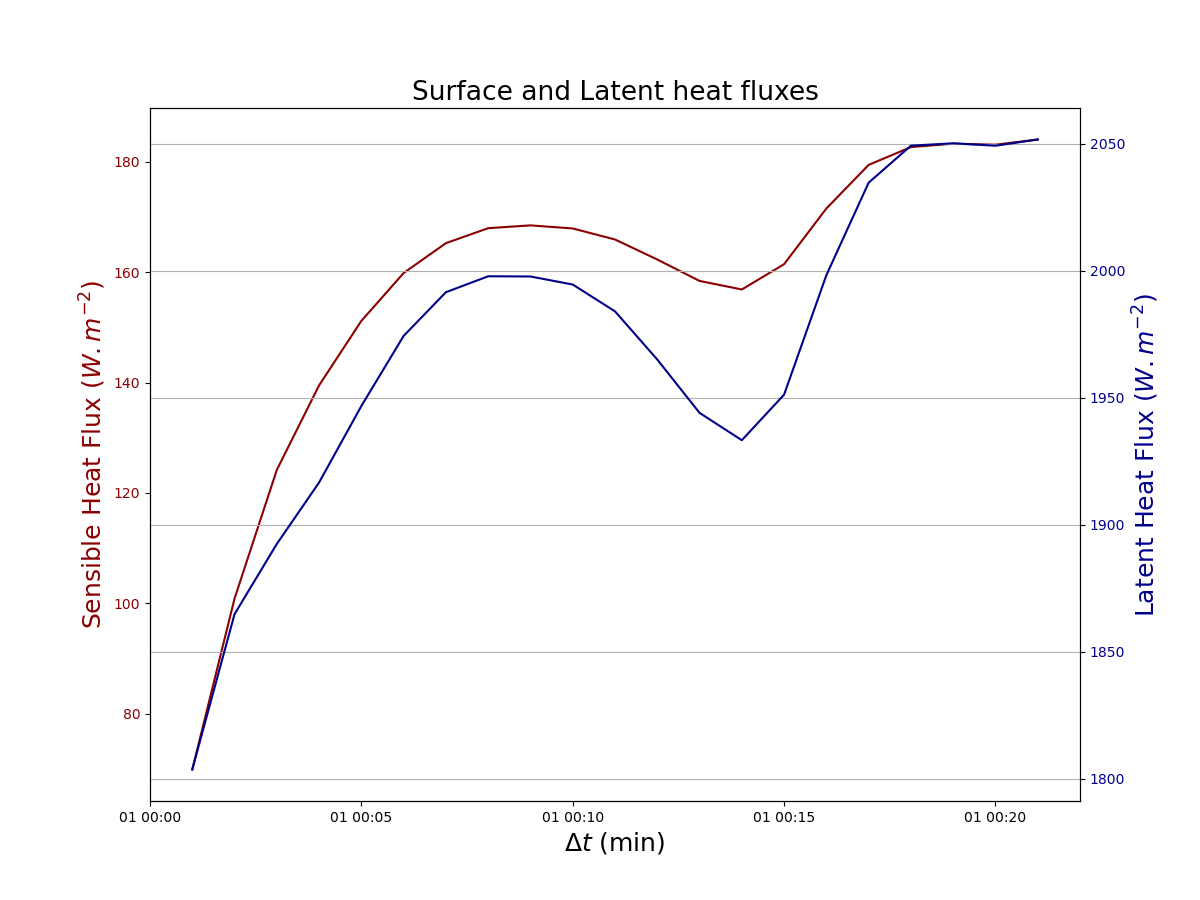
\includegraphics[width=0.85\textwidth]{FIGURES/noVAPOR/fluxes.png}
	\end{figure}
\end{frame}

\subsection{WT}
\begin{frame}{Vitesses verticales}
	petits rouleaux (dû à des flux trop forts ? ressemble à des free rolls \> pas d'influence des flux ?) faire tracé de f ? 
	\begin{figure}[t]
		\centering
		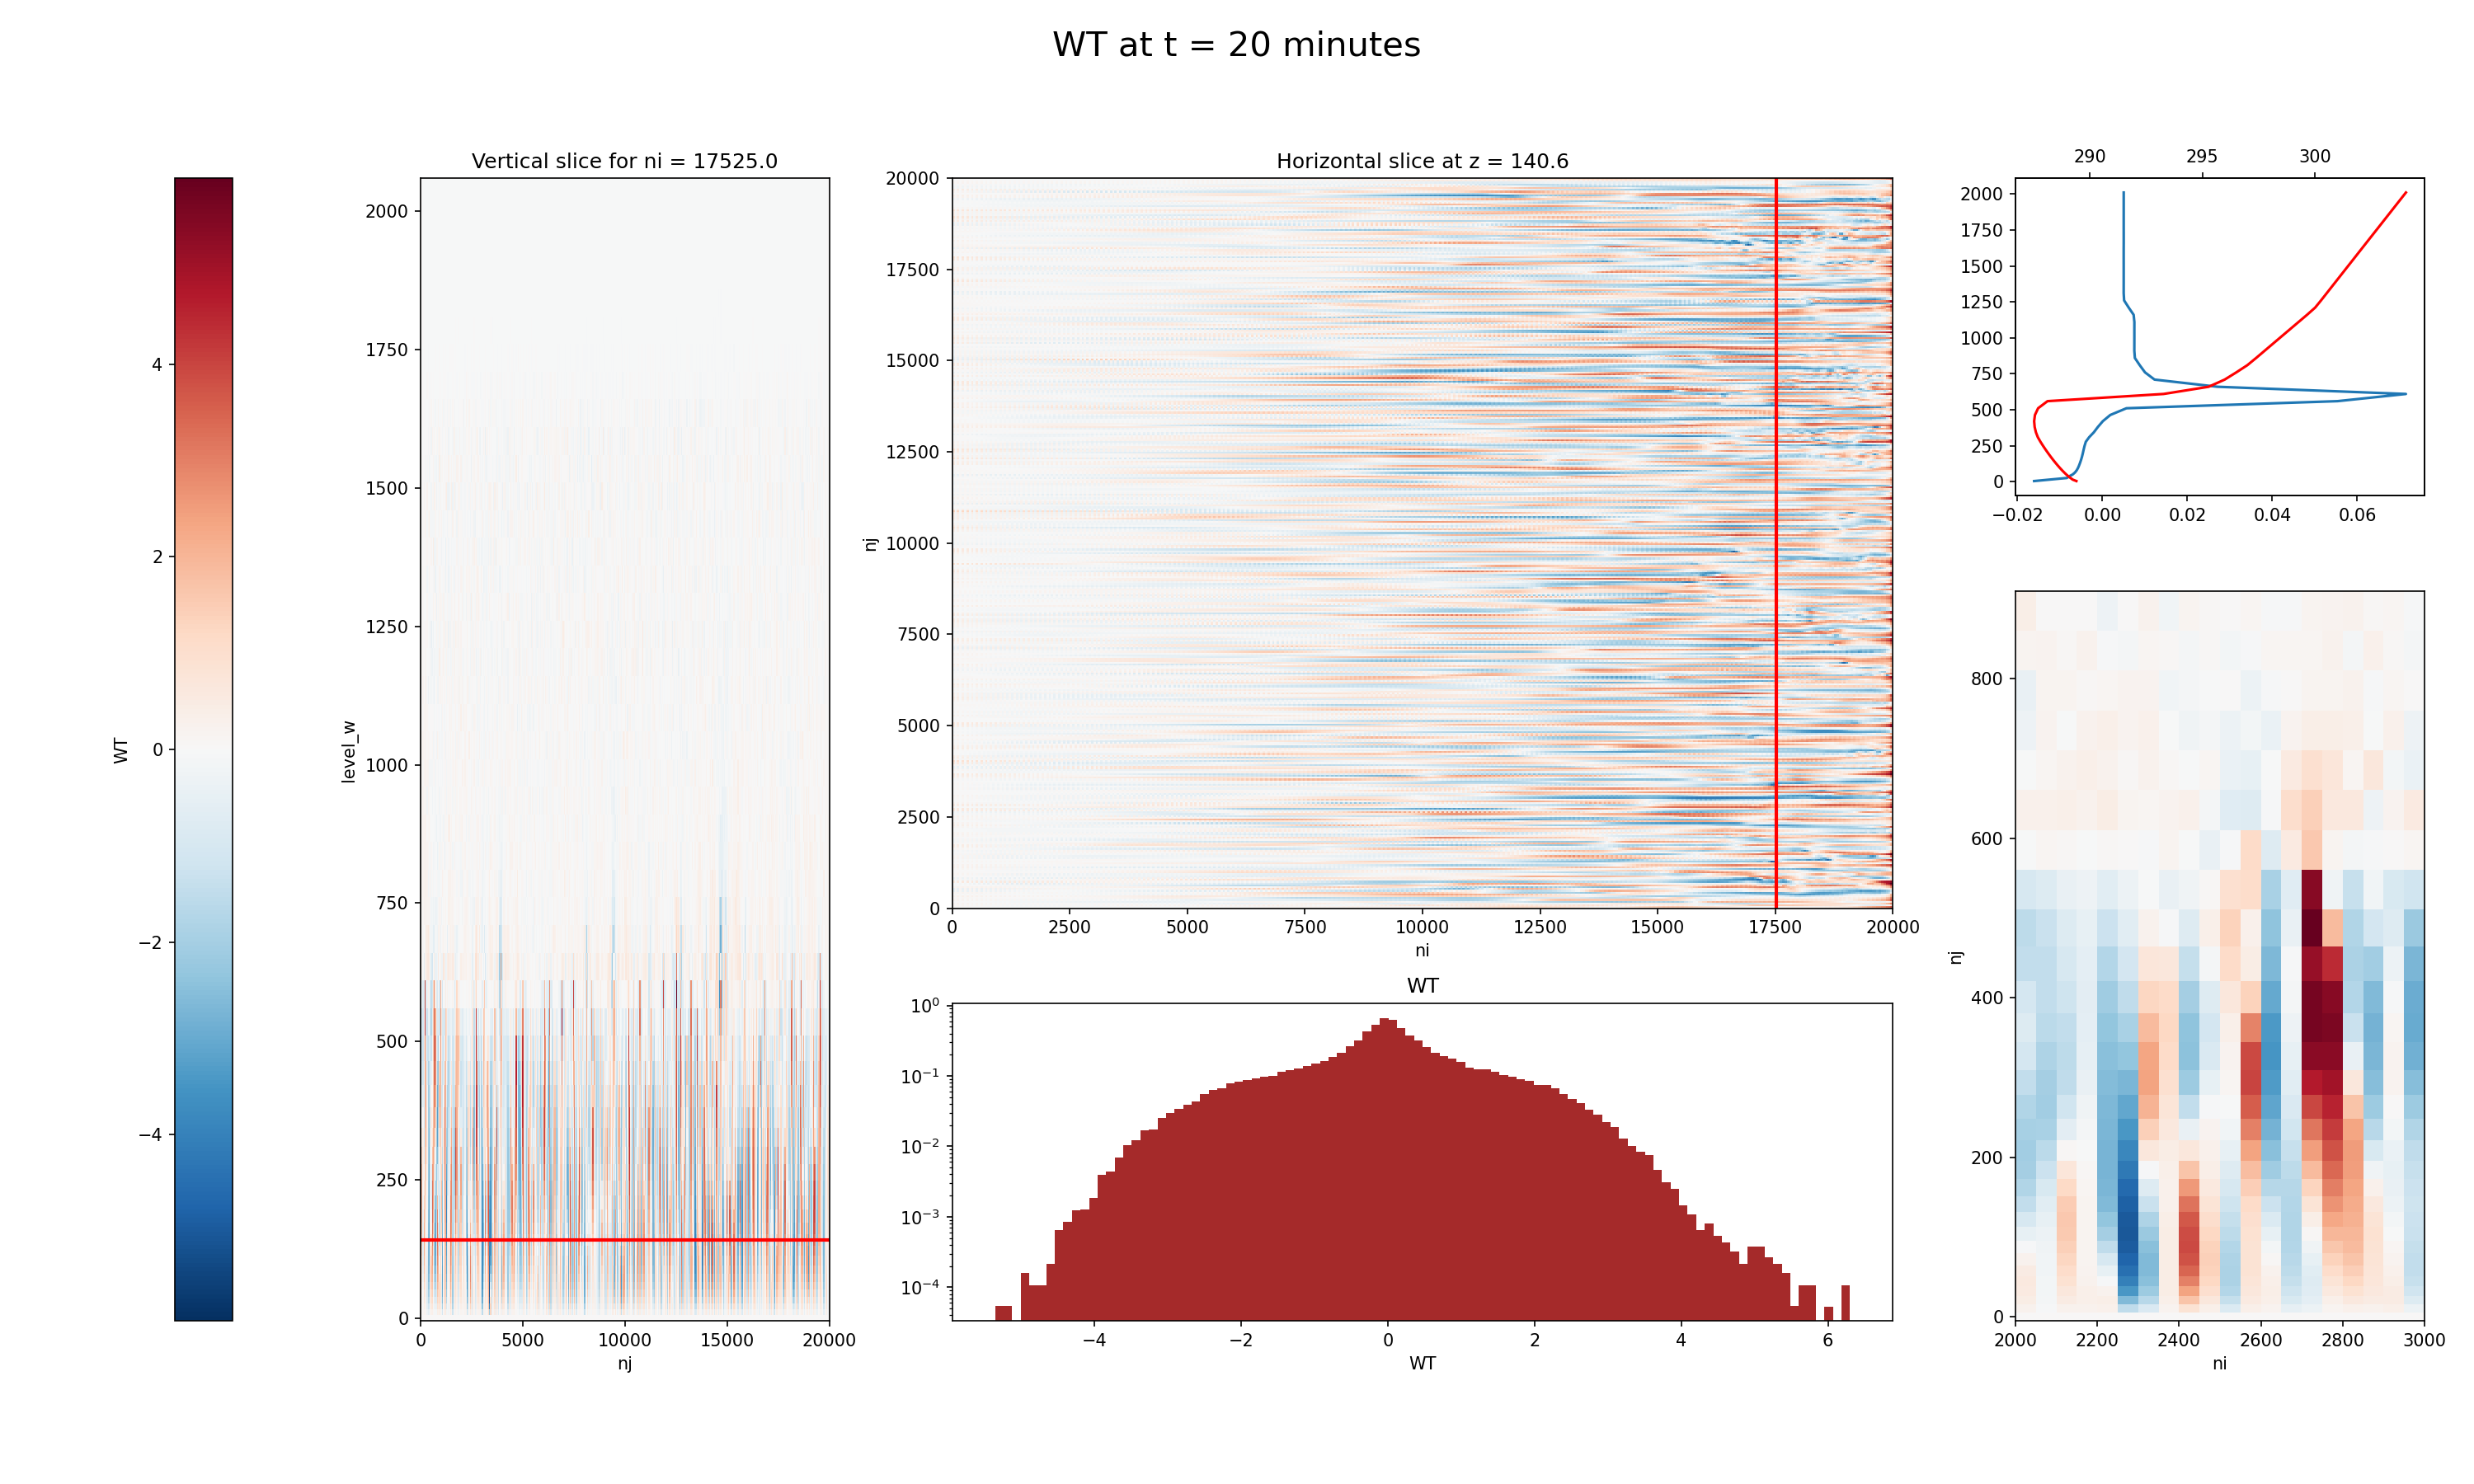
\includegraphics[width=0.85\textwidth]{FIGURES/noVAPOR/WT_ni350_t20.png}
	\end{figure}
\end{frame}

\begin{frame}{$\theta '$}

	\begin{figure}[t]
		\centering
		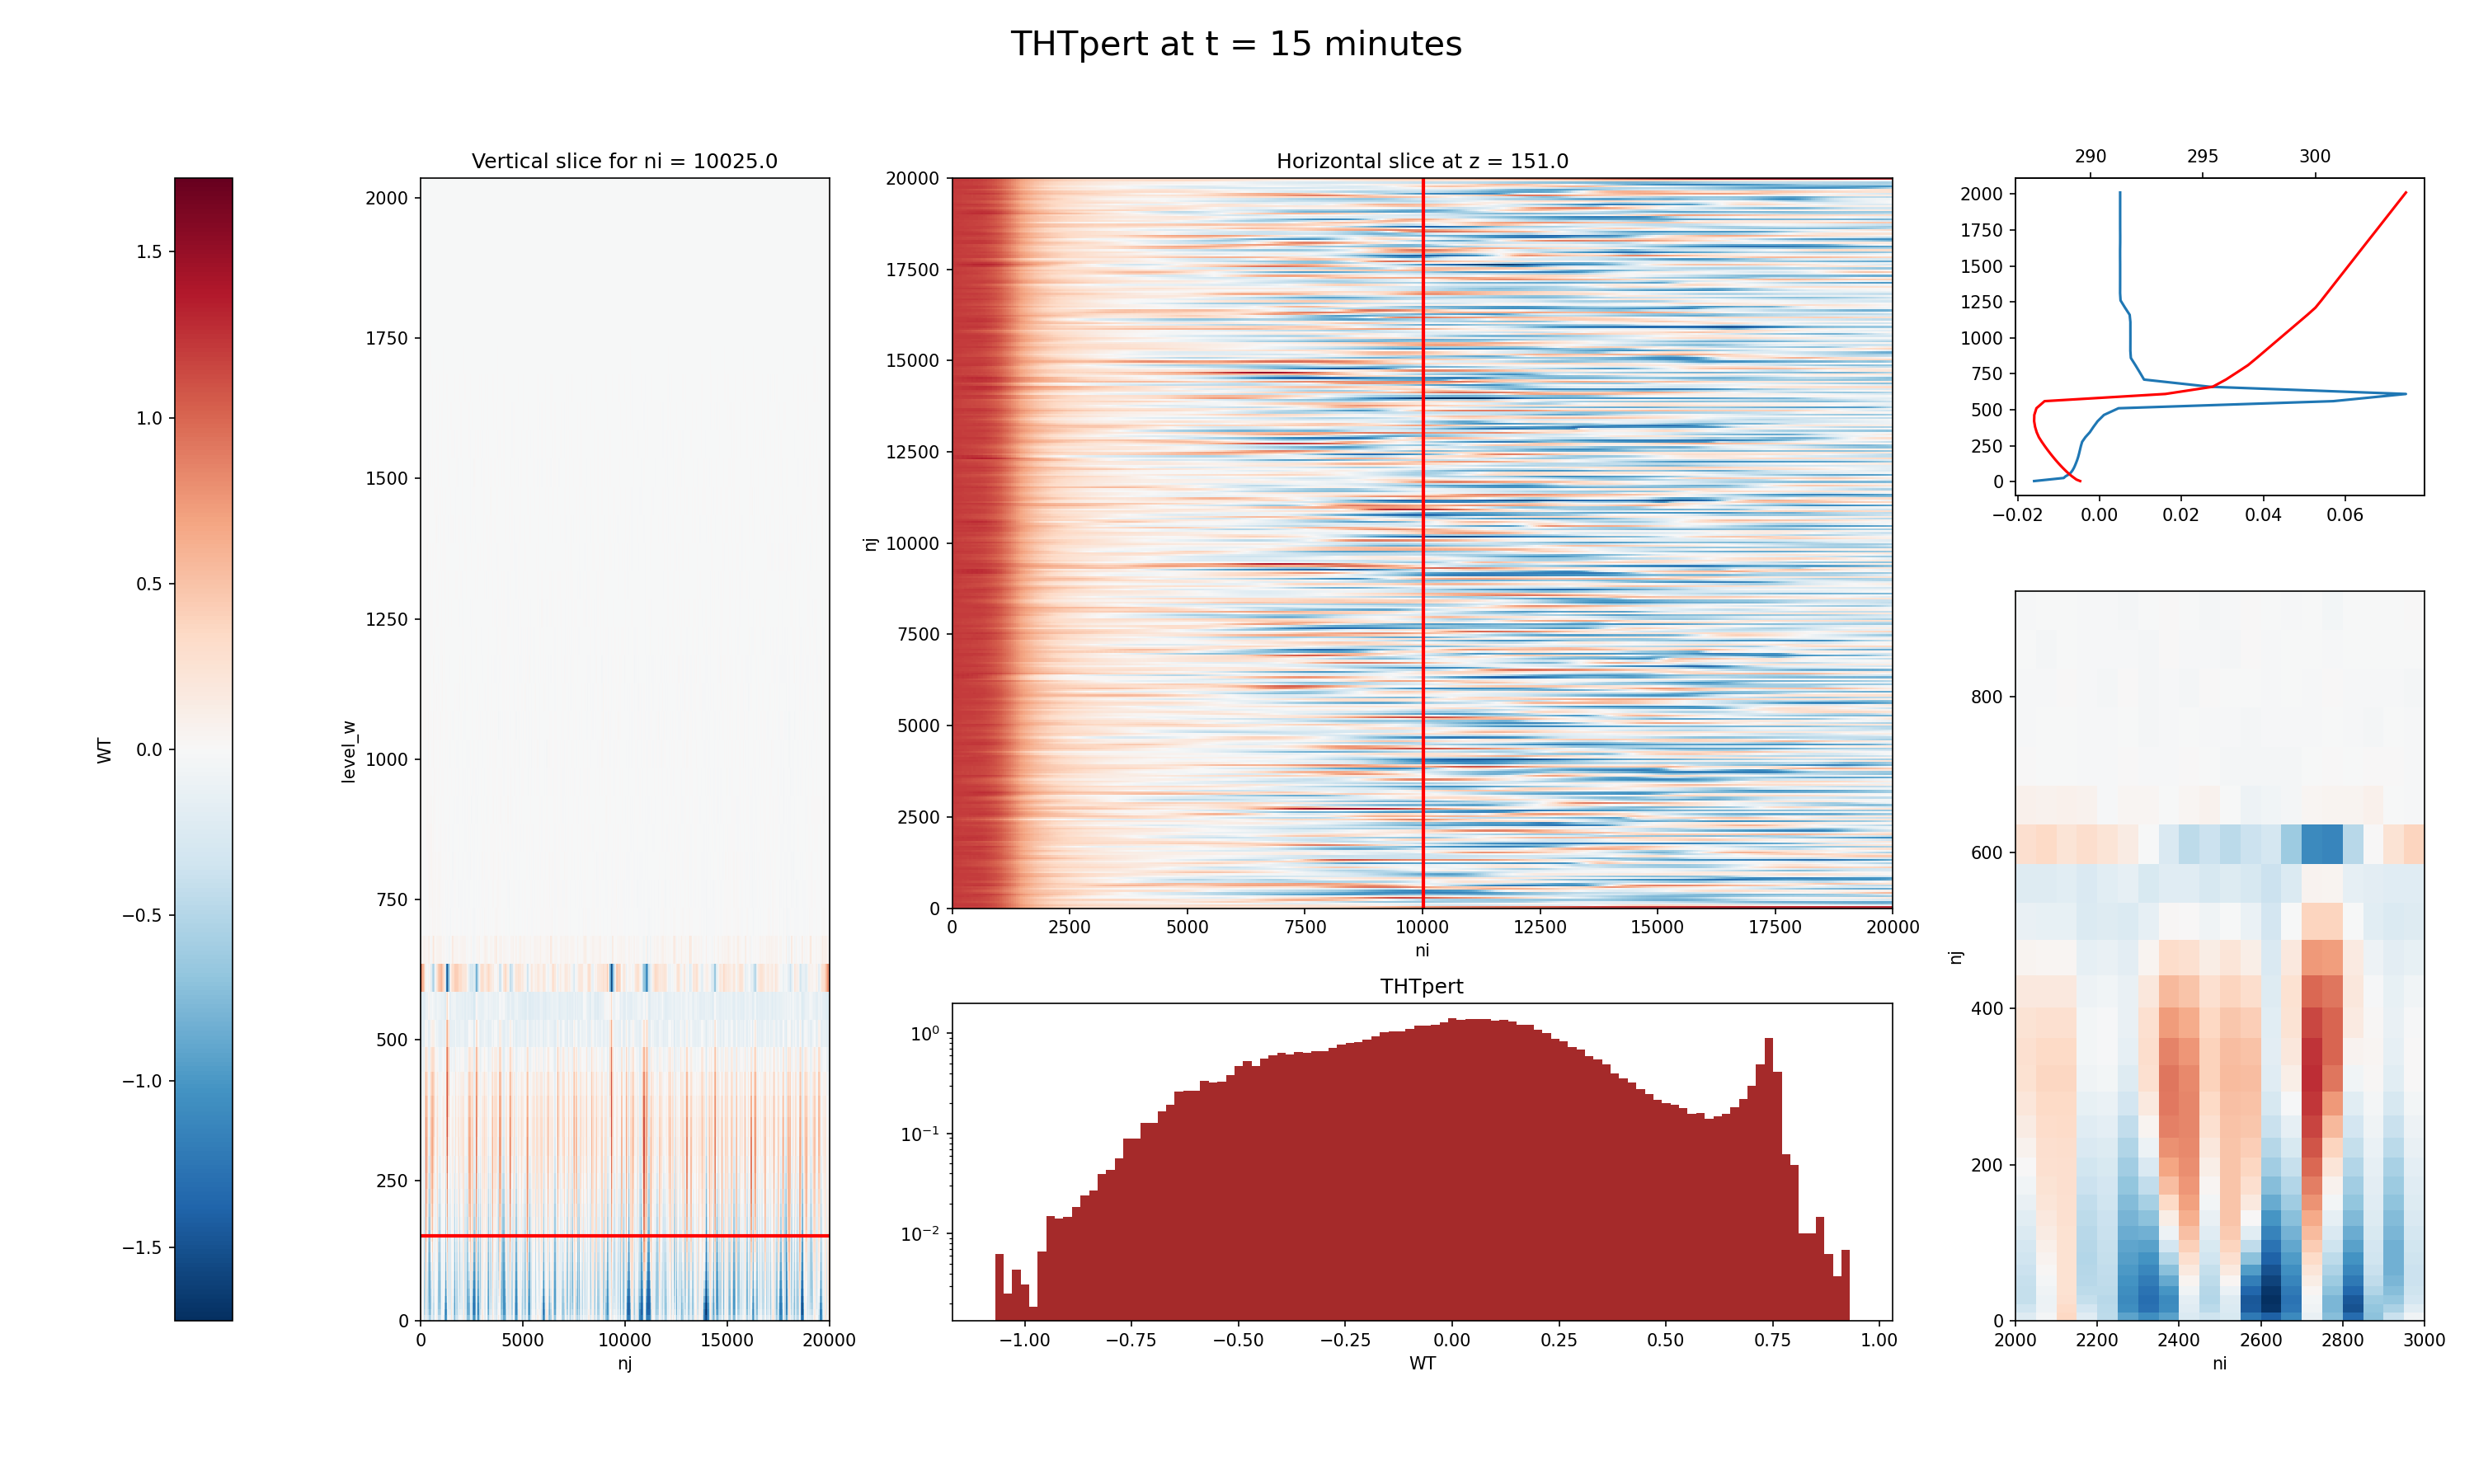
\includegraphics[width=0.85\textwidth]{FIGURES/noVAPOR/THTpert_ni200_t15.png}
	\end{figure}
\end{frame}

\begin{frame}{Prochaines pistes}
\begin{itemize}
	\item Le CT est trop grand on perd l'interet de faire des tests rapide
	\item pas vraiment des rouleaux -> jouer sur les flux ? est ce que humidité était importante ? aussi pas d'angle relatif à la direction du vent 
	\item souci c'est que pas de flux tend à stabiliser la CL
	\item pas exactement les CI de Wahiba 
\end{itemize}
\end{frame}




% Deuxième expé
\section{Simulation miniROLLS}

\begin{frame}{Simulation miniROLLS}
	
	\begin{itemize}
		\item remise bords cyclique pour accélerer le CT (conditionne surement le nombre de rouleaux mais a étudier quand on en a)
		\item mise de profils exacts de Wahiba (par contre on enleve la forte inversion )
		\item $\Delta x = \Delta y = 100m$ ; $\Delta t = 0.5 s$ pou temps de calcul correct
	\end{itemize}
	
	\begin{figure}
		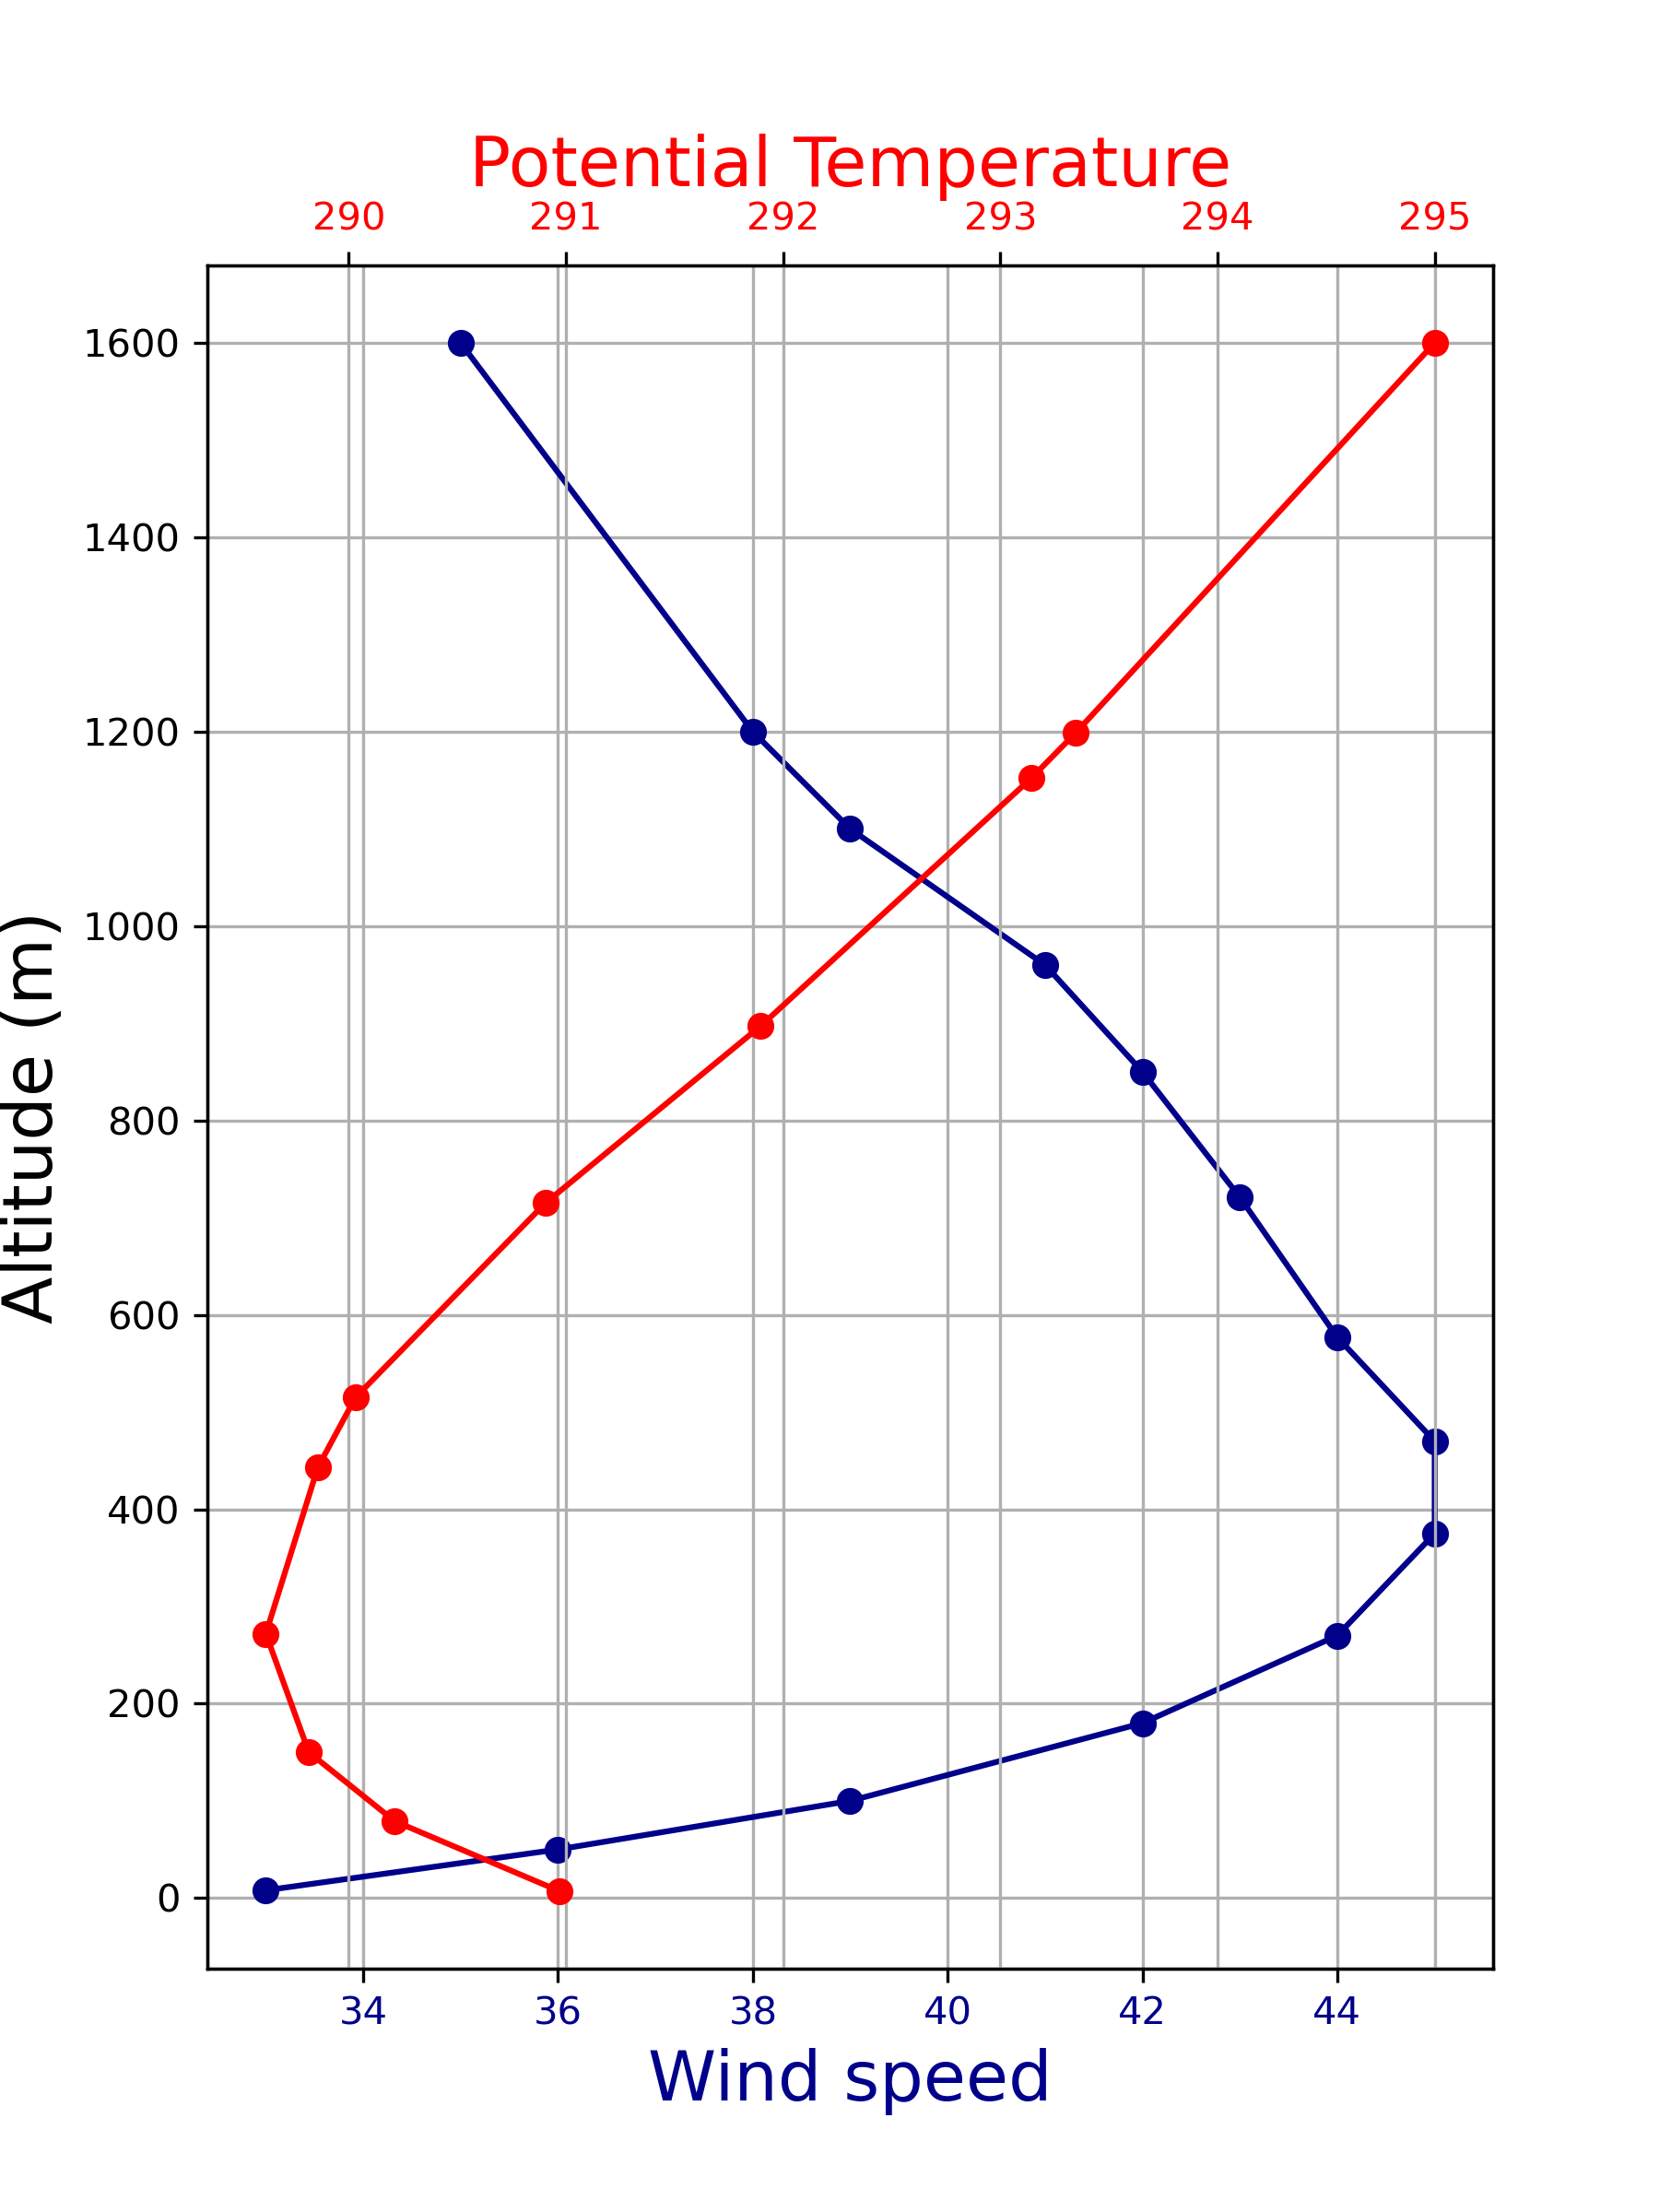
\includegraphics[width=0.4\textheight]{FIGURES/miniROLLS/inputs.png}
	\end{figure}
	
\end{frame}

\subsection{Profiles vitesses}
\begin{frame}{Profiles}
	Tjs pb des vents verticaux en altitude + CL se stabilise (peut etre du a temperétaure au sol plus faible que profil de temp dans mNH)
	\begin{figure}[t]
		\centering
		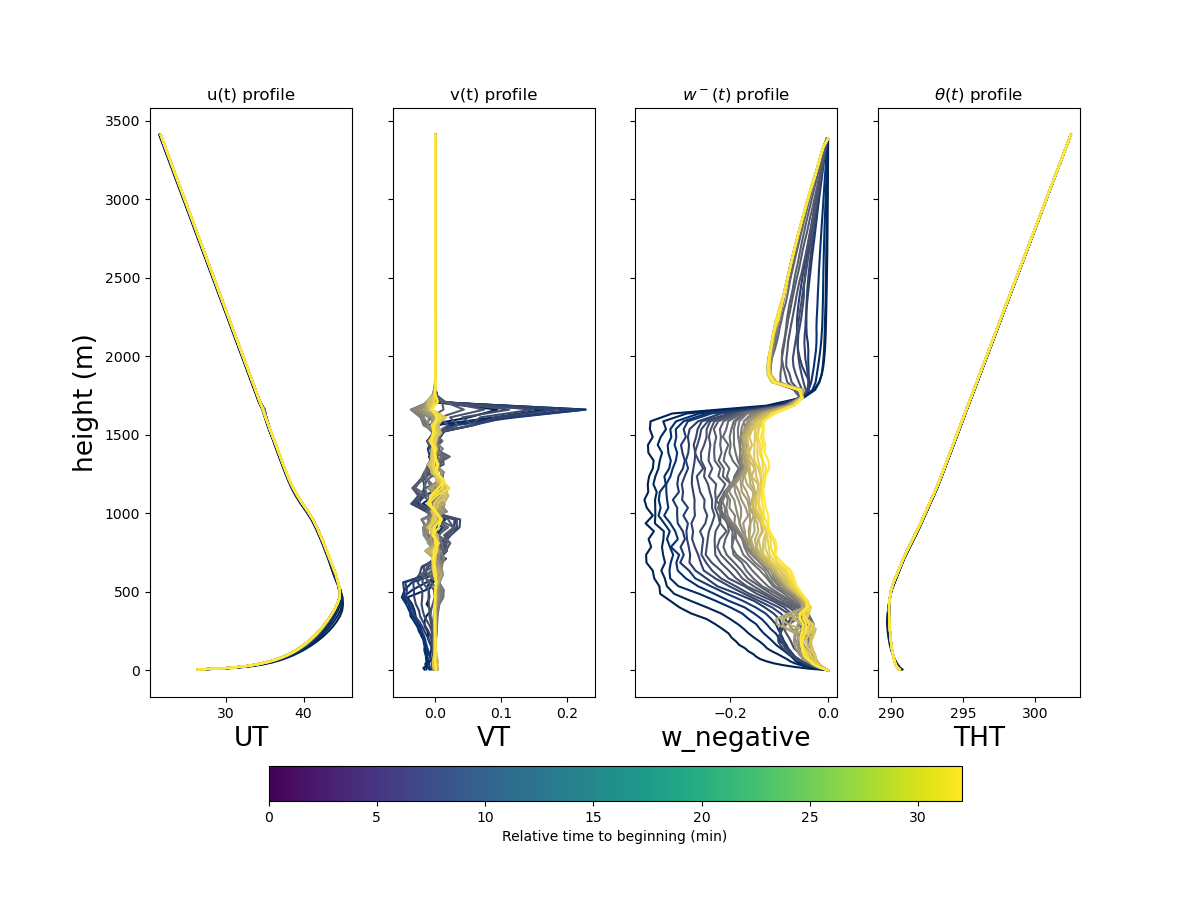
\includegraphics[width=0.8\textwidth]{FIGURES/miniROLLS/wind_profiles.png}
	\end{figure}
\end{frame}

\subsection{Flux}
\begin{frame}{Flux}
	Flux plus cohérent avec Wahiba et stables; tjs couche qui se stabilise avec un sol plus froid que la temperature du niveau 0 \hl{a changer}
	\begin{figure}[t]
		\centering
		
\includegraphics[width=0.8\textwidth]{FIGURES/miniROLLS/fluxes.png}
	\end{figure}
\end{frame}

\subsection{WT}
\begin{frame}{Vitesses verticales}
	Vitesses verticales plus faible (bonne nouvelle) mais très bruité : problème au bord droit qui se propage toujours ?  et couche d'entrainement très bruitée 
	\begin{figure}[t]
		\centering
		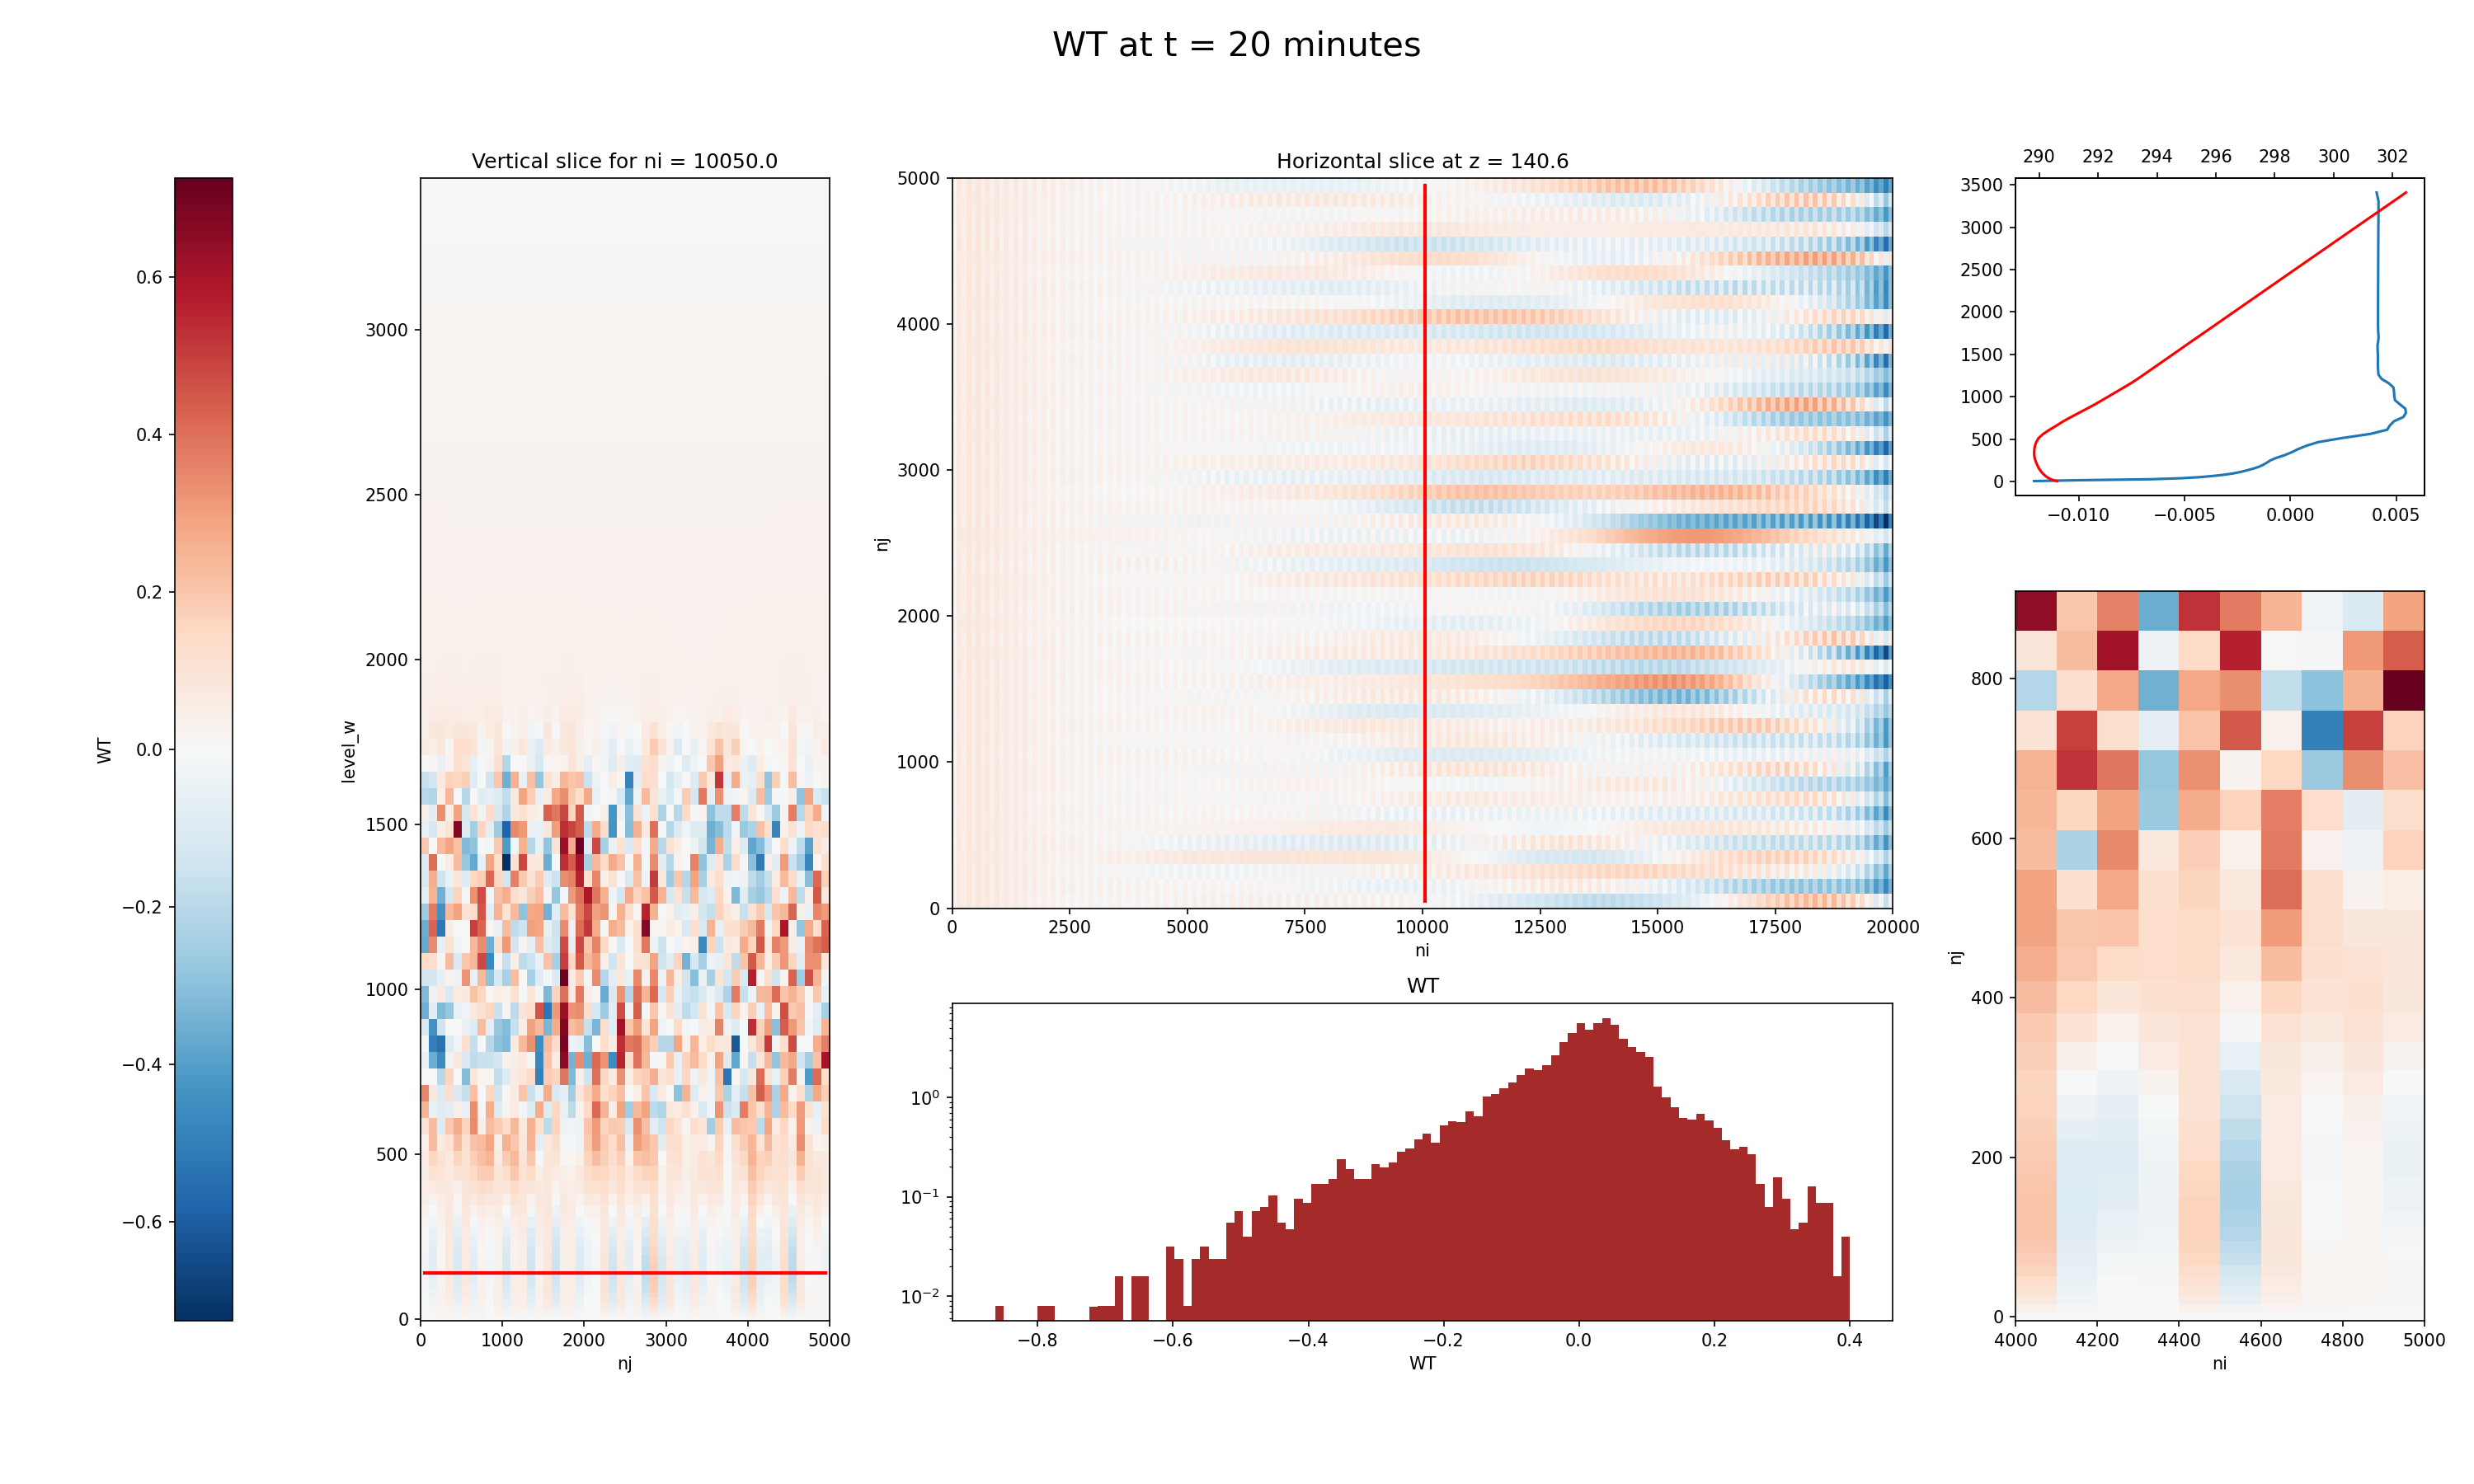
\includegraphics[width=0.8\textwidth]{FIGURES/miniROLLS/WT_ni100_t20.png}
	\end{figure}
\end{frame}

\begin{frame}{$\theta '$}
	
	\begin{figure}[t]
		\centering
		\includegraphics[width=0.85\textwidth]{FIGURES/miniROLLS/.png}
	\end{figure}
\end{frame}

\begin{frame}{Prochaines pistes}
	\begin{itemize}
		\item CT meilleur mais tjs assez grand env 4h pour 30min de simulées
		\item Toujours pas de rouleaux braiment meme si j'ai l'impression que plus proche 
		\item flux stables
		\item augmenter résolution temporelle et spatiales ? + allonger domaine selon x
	\end{itemize}
\end{frame}